\documentclass[pdf, intlimits, 9pt, unicode]{beamer}

\input{../config.tex}
\input{../header.tex}
\renewcommand{\docname}{Введение в машинное обучение}


\title[\disciplineshortname]{\docname}

\begin{document}

\maketitle

\begin{frame}<handout:0>{Содержание}\tableofcontents[pausesections]\end{frame}

\section{Введение}



\begin{frame}
	\begin{block}{Анализ данных (машинное обучение)}
	наука, изучающая способы \emph{извлечения закономерностей} из ограниченного количества примеров.
	\end{block}\pause
	\medskip
	
	Машинное обучение посвящено строгому изучению методов извлечения закономерностей из данных (см. {\color{red}\emph{математический анализ}})\pause
	
	Анализ данных -- название ремесла, направленного на решение прикладных задач (см. {\color{red}\emph{инженер}})

\end{frame}





\begin{frame}
        %Интеллект -- одна из мыслительных способностей.\pause

	\begin{block}{Искусственный интеллект}
наука и технология создания интеллектуальных машин, особенно интеллектуальных компьютерных программ; свойство интеллектуальных систем выполнять творческие функции, которые традиционно считаются прерогативой человека.
	\end{block}\pause
	\medskip

%ИИ -- это то, что когда-либо перестаёт быть ИИ (мода -- это то, что выходит из моды)\pause

	\begin{block}{Алгоритм}
	набор инструкций, описывающих порядок действий исполнителя для достижения некоторого результата
	\end{block}\pause
	\medskip

        %В творческих задачах алгоритм решения "сочиняется" в ходе поиска решения. Получается, что ИИ -- это создание достаточно гибких алгоритмов.

	\begin{block}{Экспертная система}
	компьютерная система, способная частично заменить специалиста-эксперта в разрешении проблемной ситуации
	\end{block}\pause
	\medskip

        %Алгоритмическая реализация решения искусственного интеллекта.

\end{frame}





\begin{frame}

{\color{red}Объекты} (машинного обучения) -- это абстрактные сущности (точки размещения ресторанов, графические образы, синтаксические конструкции), которыми компьютеры не умеют оперировать напрямую.

\begin{center}$O$
\end{center}\medskip\pause

Вектор всех признаков объекта $x$ называется признаковым описанием этого объекта.

\begin{center}$P = \lbrace x_1^O, \dots, x_n^O \rbrace$
\end{center}\medskip\pause

С точки зрения машинного обучения, объект тождественен своему вектору признаков.

\begin{center}
$P = O$
\end{center}

\end{frame}





\begin{frame}

Разработка признаков ({\color{red}feature engineering}) для любой задачи является одним из самых сложных и самых важных этапов анализа данных.\pause

Признаки могут быть:

\begin{itemize}
	\item бинарными (да/нет)\pause
	\item вещественными (1.43, 99.99\%)\pause
	\item категориальными (красный, оранжевый, ...)\pause
	\item ординальными (значения из неупорядоченного множества)\pause
	\item множественными (set-valued, подмножеством)
\end{itemize}

\end{frame}







\section{С учителем, без учителя}




%Обучение с учителем (Supervised learning)

\begin{frame}{Задачи обучения с учителем}
Задача машинного обучения: Имеется множество объектов (ситуаций) и множество возможных ответов (откликов, реакций).\pause

Существует некоторая зависимость между ответами и объектами, но она неизвестна.\pause

Известна только конечная совокупность прецедентов -- пар <<объект, ответ>>, называемая обучающей выборкой.\pause

На основе этих данных требуется восстановить зависимость, построить алгоритм, способный {\color{red}для любого объекта выдать достаточно точный ответ}.\pause

%Для измерения точности ответов определённым образом вводится функционал качества. 

Под учителем понимается либо сама обучающая выборка, либо тот, кто указал на заданных объектах правильные ответы. Существует также обучение без учителя, когда на объектах выборки ответы не задаются.
\end{frame}









\begin{frame}{Задачи обучения с учителем}

\textbf{Регрессия} -- задача с вещественной целевой переменной.\bigskip

\begin{center}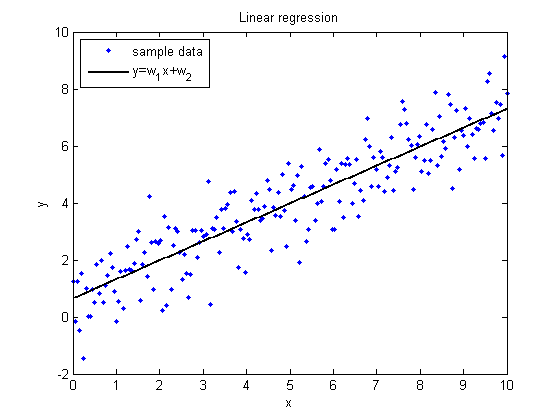
\includegraphics[width=.8\textwidth]{Regression_Analysis_Linear.png}\end{center}
\end{frame}






\begin{frame}{Задачи обучения с учителем}

$\mathbb{Y} = \{0,1\}$ -- бинарная классификация.
\bigskip

Например, мы можем предсказывать, кликнет ли пользователь по рекламному объявлению, вернет ли клиент кредит в установленный срок, сдаст ли студент сессию, случится ли определенное заболевание с пациентом (на основе его генома).

\end{frame}




\begin{frame}
\begin{center}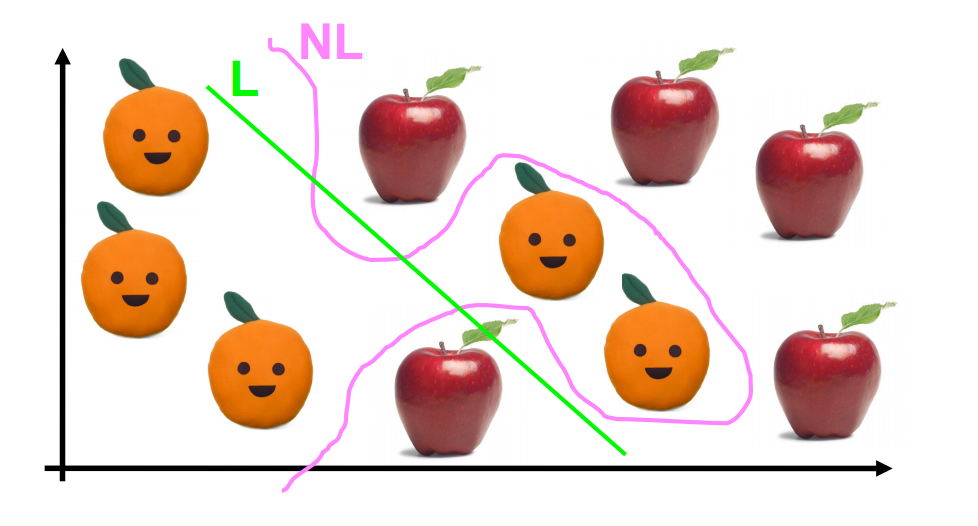
\includegraphics[width=\textwidth]{ML_surfaces.png}\end{center}
\end{frame}




\begin{frame}{Задачи обучения с учителем}

$\mathbb{Y} = \{1 ... M\}$ -- многоклассовая (multi-class) классификация.
\bigskip

Примером может служить определение предметной области для научной статьи (математика, биология, психология и т.д.).
\end{frame}






\begin{frame}{Задачи обучения с учителем}

$\mathbb{Y} = \{0,1\}^M$ -- многоклассовая классификация с пересекающимися классами (multi-label classification).
\bigskip

Примером может служить задача медицинской диагностики, где для пациента нужно определить набор заболеваний, которыми он страдает.
\end{frame}





\begin{frame}{Задачи обучения с учителем}

\textbf{Ранжирование} -- задача, в которой требуется восстановить порядок на некотором множестве объектов.
\bigskip

Основным примером является задача ранжирования поисковой выдачи, где для любого запроса нужно отсортировать все возможные документы по релевантности этому запросу.
\end{frame}







\begin{frame}{Частичное обучение}

\textbf{Частичное обучение} (semi-supervised learning) -- задача, в которой для одной части объектов обучающей выборки известны и признаки, и ответы, а для другой только признаки.
\bigskip

Такие ситуации возникают, например, в медицинских задачах, где получение ответа является крайне сложным (например, требует проведения дорогостоящего анализа).
\end{frame}





\begin{frame}{Обучение без учителя}

Класс задач, где ответы неизвестны или вообще не существуют, и требуется найти некоторые закономерности в данных лишь на основе признаковых описаний.\pause

\textbf{Кластеризация} -- задача разделения объектов на группы, обладающие некоторыми свойствами.\pause
\bigskip

Примером может служить кластеризация документов из электронной библиотеки или кластеризация абонентов мобильного оператора.
\end{frame}




\begin{frame}
\begin{center}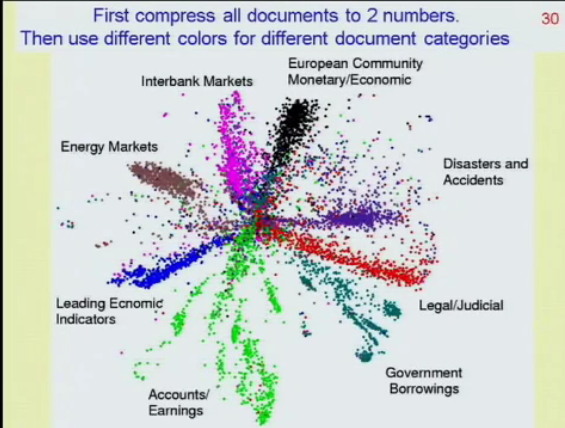
\includegraphics[width=\textwidth]{s1.png}\end{center}
\end{frame}




\begin{frame}
\begin{center}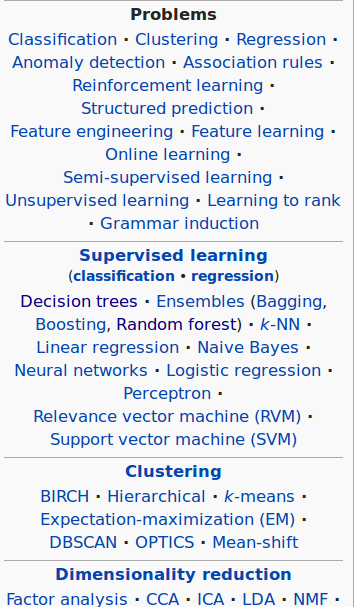
\includegraphics[width=\textwidth]{s2.png}\end{center}
\end{frame}





\begin{frame}{Обучение без учителя}
Класс задач, где требуется найти некоторые закономерности в данных лишь на основе признаковых описаний. Правильные ответы в обучающей выборке не даны или вообще не существуют.\pause

\textbf{Оценивание плотности} -- задача приближения распределения объектов.\pause
\bigskip

Примером может служить кластеризация документов из
электронной библиотеки или кластеризация абонентов мобильного оператора.
\end{frame}





\section{Построение моделей обучения}





\begin{frame}{Функционал качества}

Нашей задачей является построение функции $a : X \rightarrow Y$, которая для любого объекта будет предсказывать ответ.\pause

Такая функция называется алгоритмом или моделью (hypothesis).\pause

Понятно, что нам подойдет далеко не каждый алгоритм -- например, вряд ли мы извлечем какую-то выгоду из алгоритма $a(x) = 0$, независимого от признаков.
\end{frame}

\begin{frame}{Функционал качества}
Чтобы формализовать соответствие алгоритма нашим ожиданиям, нужно ввести \emph{функционал качества}, измеряющий качество работы алгоритма. Крайне популярным функционалом в задаче регрессии является среднеквадратичная ошибка (mean squared error, MSE):

$$Q (a, X^l) = \frac{1}{l} \sum_{i=1}^{l}{(a(x_i) - y_i)^2}$$\pause

Удобства: дифференцируемость и простота описания.

Именно функционал качества определяет, какой алгоритм является лучшим, поэтому с плохим функционалом...
\end{frame}






\begin{frame}{Построение алгоритма обучения}
Как только функционал качества зафиксирован, можно приступать к построению алгоритма $a(x)$.\pause

Как правило, для этого фиксируют некоторое семейство алгоритмов $\mathcal{A}$, и пытаются выбрать из него алгоритм, наилучший с точки зрения функционала.\pause

В машинном обучении было изобретено большое количество семейств
алгоритмов, и самым простым и тщательно изученным является \textbf{семейство линейных моделей}, которые дают предсказание, равное линейной комбинации признаков:

$$\mathcal{A} = \{ a(x) = w_0 + w_1 x^1 + \dots + w_d x^d | w_0, w_1, \dots w_d \in \mathbb{R} \}$$

\end{frame}





\begin{frame}

$$\mathcal{A} = \{ a(x) = w_0 + w_1 x^1 + \dots + w_d x^d | w_0, w_1, \dots w_d \in \mathbb{R} \}$$

$x_i$ -- значение $i$-го признака у объекта $x$.\pause

Лучшая из таких моделей будет выбираться минимизацией MSE-функционала:

$$\frac{1}{l} \sum_{i=1}^{l}{ \left ( w_0 + \sum_{j=1}^{d}{w_j x_i^j - y} \right )^2 } \rightarrow \underset{w_0, w_1, \dots, w_d}{min} $$\pause

Процесс поиска оптимального алгоритма называется \emph{обучением}.

\end{frame}






\begin{frame}<handout:0>
Обычно необходимо переработать данные перед началом построения модели.\pause

\begin{itemize}
\item \textbf{Нормализация:} Некоторые модели хорошо работают только при выполнении определенных требований. Так, для линейных моделей крайне важно, чтобы признаки были нормированными, то есть измерялись в одной шкале (вычитание среднего и деление на дисперсию каждого столбца в матрице "объекты/признаки".\pause
\item \textbf{Фильтрация:} Бывает, что в выборку попадают выбросы -- объекты, которые не являются корректными примерами из-за неправильно посчитанных признаков, ошибки сбора данных. Их наличие может сильно испортить модель.\pause
\item \textbf{Переобучение:} {Некоторые признаки могут оказаться шумовыми, то есть не имеющими никакого отношения к целевой переменной и к решаемой задаче. Примером, скорее всего, может служить признак <<фаза луны в день первого экзамена>> в задаче предсказания успешности прохождения сессии студентом.}
\end{itemize}

\end{frame}





\begin{frame}<beamer:0>

Зачастую возникает потребность в предобработке данных до начала построения модели.\pause

Здесь может идти речь о некотором ряде манипуляций:

\textbf{Нормализация.} {Некоторые модели хорошо работают только при выполнении определенных требований. Так, для линейных моделей крайне важно, чтобы признаки были нормированными, то есть измерялись в одной шкале. Примером способа нормировки данных является вычитание среднего и деление на дисперсию каждого столбца в матрице <<объекты-признаки>>.}
\end{frame}





\begin{frame}<beamer:0>

\textbf{Фильтрация.} {Бывает, что в выборку попадают выбросы -- объекты, которые не являются корректными примерами из-за неправильно посчитанных признаков, ошибки сбора данных. Их наличие может сильно испортить модель.}

\textbf{Переобучение.} {Некоторые признаки могут оказаться шумовыми, то есть не имеющими никакого отношения к целевой переменной и к решаемой задаче. Примером, скорее всего, может служить признак <<фаза луны в день первого экзамена>> в задаче предсказания успешности прохождения сессии.}
\end{frame}







\begin{frame}{Переобучение (overfitting)}

Простейшая предобработка данных может радикально улучшить качество итоговой модели.

Пример. Допустим, что мы выбрали очень богатое семейство алгоритмов, состоящее из всех возможных функций: $\mathcal{A} = {a : X \rightarrow Y}$.\pause

В этом семействе всегда будет алгоритм, не допускающий ни одной
ошибки на обучающей выборке, который просто запоминает ее:\pause

$$a(x) = \left \{  \begin{matrix} y_i, & x = x_i\\  0, & x \in X^l\end{matrix}\right .$$

Очевидно что для любого нового объекта, алгоритм покажет нулевой прогноз -- модель переобучена.
\end{frame}






\begin{frame}{Идея для борьбы с переобучением}

В нашем примере переобучение возникло из-за большой сложности семейства -- алгоритмом могла оказаться любая функция. \pause

Очевидно, что если бы мы ограничили себя только линейными моделями, то итоговый алгоритм уже не смог
бы запомнить всю выборку.\pause

Таким образом, можно бороться с переобучением путём контроля \emph{сложности семейства алгоритмов} -- чем меньше у нас данных для обучения, тем более простые семейства следует выбирать.
\end{frame}






\begin{frame}{Отложенная выборка}

После того, как модель построена, нам нужно оценить, насколько хорошо она будет работать на новых данных.\pause

Для этого, например, можно в самом начала отложить часть обучающих объектов и не использовать их при построении модели.\pause

Тогда можно будет измерить качество готовой модели на этой отложенной выборке, получив тем самым оценку того, насколько она готова к работе на новых данных.\pause

Существуют и более сложный класс методов, называемый кросс-валидацией...
\end{frame}






\begin{frame}{Решение задачи анализа данных}
	\begin{center}
\leftright{\textbf{Проектировщик}}{\textbf{Пользователь}}
\leftright{Постановка задачи}{}\pause
\leftright{$\Downarrow$}{}
\leftright{Выделение признаков}{}\pause
\leftright{$\Downarrow$}{}
\leftright{Формирование выборки}{}\pause
\leftright{$\Downarrow$}{}
\leftright{Выбор метрики качества}{}\pause
\leftright{$\Downarrow$}{}
\leftright{Подготовка/переработка данных}{}\pause
\leftright{$\Downarrow$}{}
\leftright{Построение алгоритма обучения}{}\pause
\leftright{}{\emph{Обучение}}\pause
\leftright{Оценка качества модели}{}\pause
\leftright{}{\emph{Использование}}
	\end{center}
\end{frame}




%\begin{frame}{Система обработки языка}\begin{center}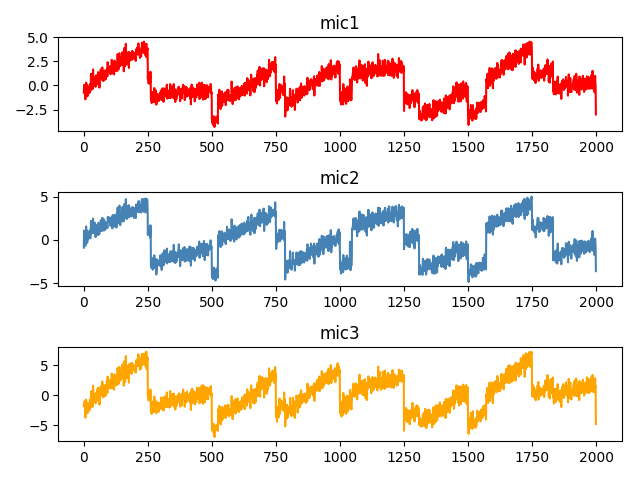
\includegraphics[width=\textwidth]{3.png}\end{center}\end{frame}





%\section{Нисходящий анализ}\stepcounter{subsection}\repeatSectionTitle
%\begin{center}Пример UPPAAL + Python\end{center}
%\begin{frame}\begin{center}\includegraphics[width=.9\textwidth]{10.png}\end{center}\end{frame}



\repeatSectionTitle[Спасибо за внимание!]

\end{document}
